\chapter{Il PDF e l'Estrazione delle informazioni}
Prima di poter estrarre dati utili dai documenti PDF è necessario operare delle trasformazioni o delle rappresentazioni, dato che, per natura del PDF non vi sono dei dati utili al nostro scopo direttamente leggibili.

\section{Cosa sono i PDF?}
PDF è un acronimo che sta per \textit{Portable Document Format} è uno formato standard creato nel 1993 allo scopo di rappresentare documenti testuali o con immagini indipendentemente dall'hardware o dal software che usato per generare o visualizzare il documento stesso. I file costruiti in questo formato sono rappresentati tramite una sequenza di caratteri ASCII, all'interno possiamo individuare quattro strutture:

\begin{itemize}
	\item Header
	\item Body
	\item Cross-Reference Table
	\item Trailer
\end{itemize}
Ciò che viene presentato visivamente all'utente è contenuto nella sezione \texttt{body} del PDF, su questo flusso di caratteri si opera per ottenere le informazioni volute.
\newpage
\section{Tecniche di estrazione}
Le tecniche di estrazione sono principalmente due:
\begin{itemize}
	\item Conversione in formati testuali
	\item Lettura diretta del flusso \texttt{Body}
\end{itemize}

Nel primo caso si cerca di convertire (tramite librerie o servizi appositi) il documento in un file di testo dove poter effettuare l'estrazione. Questo metodo è stato scartato durante i test d'implementazione preliminari per via del risultato insoddisfacente, difatti i tentativi di conversione (con strumenti già esistenti e librerie dedicate) non riuscivano a convertire le tabelle in testo ma venivano generate delle immagini. 
Non è stato possibile utilizzare librerie dedicate all'estrazione di tabelle poiché gli antibiogrammi hanno una posizione fissa.
Nel secondo caso la realizzazione di un prodotto completo avrebbe richiesto studi molto più lunghi e fuori dallo scopo della tesi.
\section{La libreria utilizzata}
In un primo momento si è tentato di utilizzare la stessa libreria responsabile della generazione dei documenti, ma limitazioni di licenza e funzionalità hanno favorito la concorrente open-source Apache PDFBox che si è rivelata oltretutto più versatile e adatta allo scopo prefissato.
\section{L'approccio iniziale e le problematiche}
Il primo approccio si è basato sulla semplice estrazione del testo linea per linea dai referti con l'applicazione di specifiche regex. 
Avendo inizialmente soltanto un referto su cui effettuare i test non è apparso subito l'evidente problema sorto in seguito con gli antibiogrammi multi-microrganismo.
L'algoritmo di estrazione era dunque costituito dai seguenti passaggi:
\begin{enumerate}
\item Scorrere la lista fino a trovare la stringa corrispondente alla parola "Microrganismo 1" seguito dal nome del microrganismo
\item Scorrere di 2 posizioni (equivalenti a saltare la riga "Microrganismo 1" e "ANTIBIOTICO MIC")
\newpage
\item Verificare ed estrarre le informazioni riguardo alla riga della tabelle tramite la seguente regex:
\begin{figure}[h!]
	\centering
	
\includegraphics[width=.99\columnwidth]{images/regex.png}
	\caption{\textit{Regex per l'estrazione delle righe della tabella}}
	\label{fig:content_multi_1}
\end{figure}
\item Ripetere fino all'arrivo della riga contenente la legenda.
\end{enumerate}

Per poter estrarre le informazioni da tabelle con più microrganismi è possibile modificare la regex ripetendo la seconda riga (la parte col gruppo MIC e Sensibilità) quante volte sono i microrganismi individuati.
Questa soluzione però fallisce nel caso di coppia di celle vuote (che significa analisi antibiotica non condotta per tale microrganismo).
\newline
\begin{figure}[h!]
	\centering
	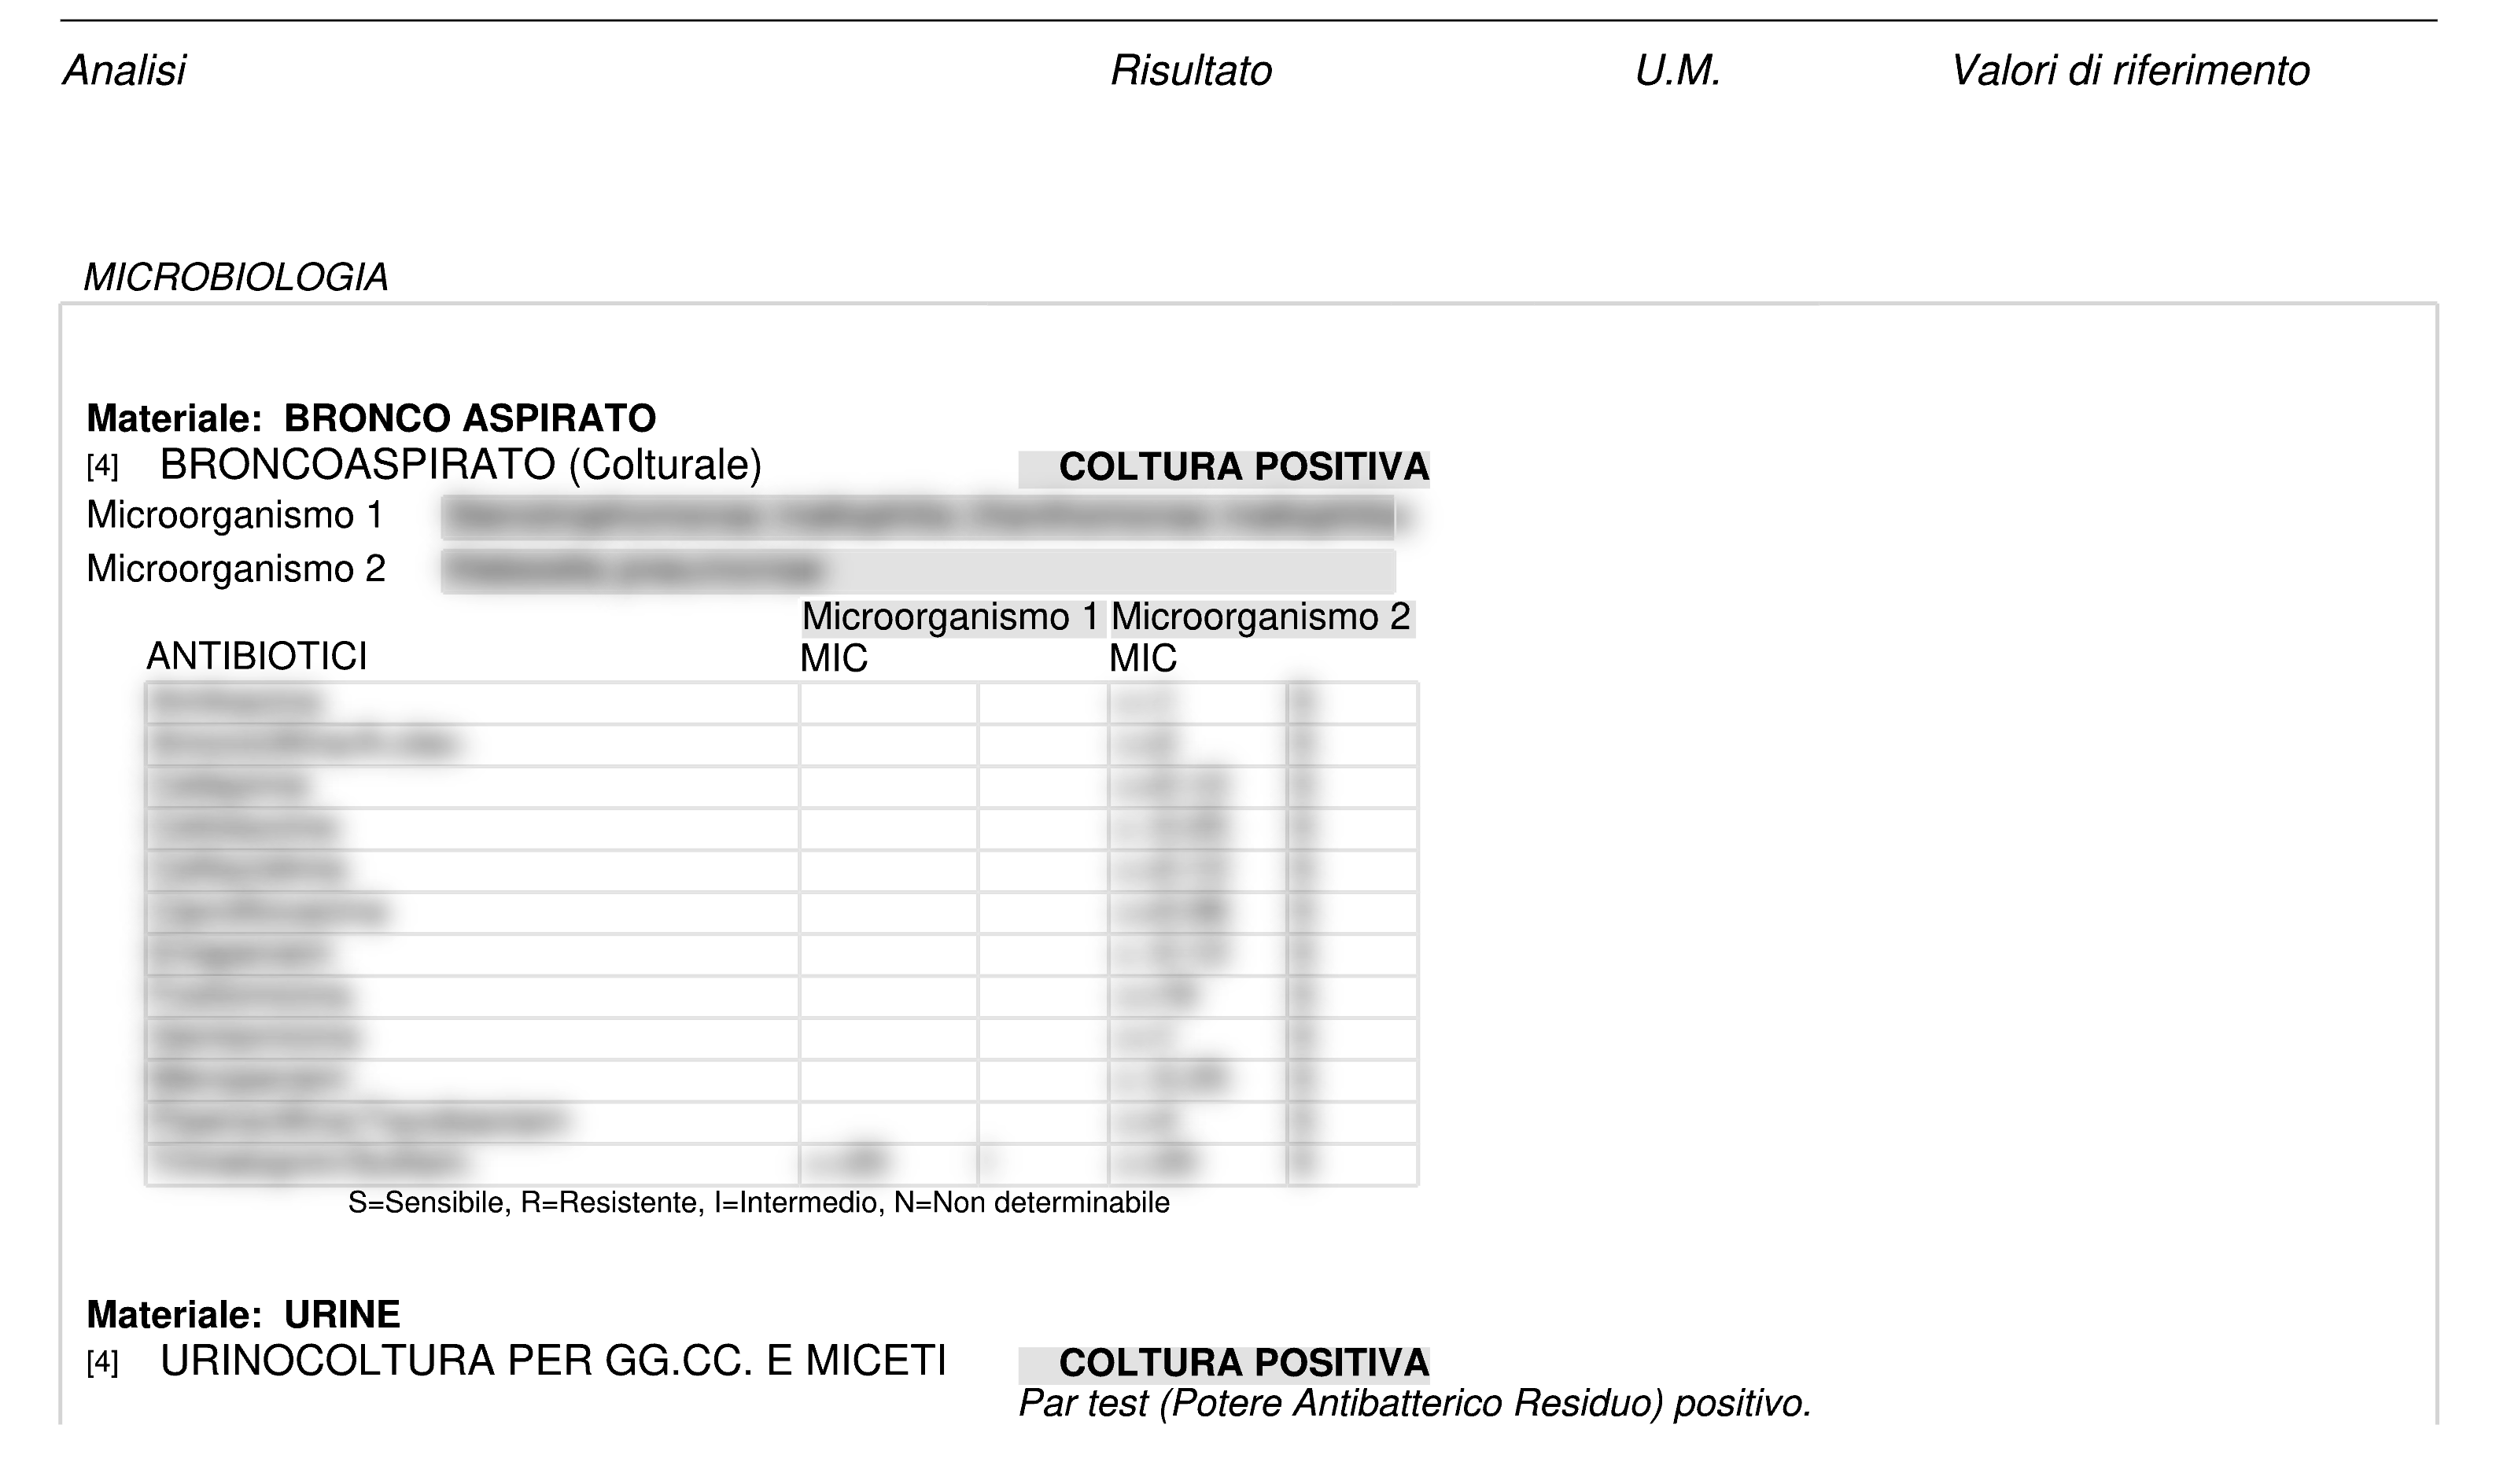
\includegraphics[width=.99\columnwidth]{images/content_multi_p1.png}
	\caption{\textit{Tabella con più microrganismi}}
	\label{fig:content_multi_1}
\end{figure}
\newline
Per esempio, nella tabella mostrata nella figura \ref{fig:content_multi_1} soltanto l'ultima riga potrà estrarre dei risultati validi tramite modifica delle regex, che risulterebbe la seguente:
\begin{figure}[h!]
	\centering
	
\includegraphics[width=.99\columnwidth]{images/regex_2.png}
	\caption{\textit{Regex per l'estrazione delle righe della tabella}}
	\label{fig:content_multi_1}
\end{figure}
Dove \textit{NR\_MICRO} è da sostituire col numero di microrganismi.
\section{Il secondo approccio}
Il secondo approccio, che apporta la correzione più significativa rivede completamente la logica di estrazione e aggiunge delle modifiche alla libreria PDFBox.
Il concetto fondamentale di quest'approccio è un estrazione "ibrida" ossia si ricerca l'inizio della tabella come nel metodo precedente, ma l'estrazione dei dati vera è propria viene effettuata calcolando la posizione delle varie celle.
\newline
Infatti anche se la posizione e la dimensione della tabella non è costante, le celle invece lo sono, permettendo un calcolo preciso della loro posizione e conseguente estrazione.
\subsection{Modifica della libreria}
Per ottenere la posizione degli elementi si è proceduto ad estendere la classe \textit{PDFTextStripper} della libreria aggiungendo prima una lista di oggetti di tipo \texttt{<string, List<TextPosition>}, ogni oggetto di questa lista è composto da una coppia chiave-valore in cui la chiave è una qualsiasi parola estratta e la chiave è una lista di posizioni in cui ogni lettera ha una sua coordinata.
Come seconda cosa è stato modificato il metodo \textit{writeString} in modo che inserisse nella lista prima citata queste nuove informazioni lasciando però inalterato il resto delle istruzioni.
\newline
\subsection{Localizzazione delle celle}\label{Algoritmo finale}
Una volta generate queste informazioni è possibile rappresentare l'algoritmo come segue:
\begin{enumerate}
	\item Si effettua una prima ricerca della tabella in modo analogo al metodo precedente
	\item Si continua a scorrere la lista e si tiene traccia del numero di microrganismi presenti nella tabella trovata
	\item Finita l'enumerazione dei microrganismi, si inizia a scorrere la nuova lista della classe modifica fino a trovare la parola chiave "ANTIBIOTICI", seguita da tante stringhe "MIC" quanti sono i microrganismi
	\item L'elemento puntato dalla lista sarà il nome dell'antibiotico, da qui si calcolano le dimensioni e le posizioni delle celle MIC e Sensibilità
	\item Definiamo tre "regioni" (dei rettangoli in cui operare), una per estrarre il nome dell'antibiotico alla linea selezionata, una per quella successiva e una per la legenda
	\item Si tenta la prima estrazione del testo, seguita poi, per ogni microrganismo dai seguenti passi:
	\begin{enumerate}
		\item Si calcola la cella MIC le cui coordinate saranno: distanza colonna antibiotico $ + 156 + $ (n° microrganismo)$*42$
		\item Discorso analogo per la cella Sensibilità che ha coordinate : distanza colonna MIC $ + $ (n° microrganismo) $*30*$
		\item Vengono definite altre due regioni, si tenta l'estrazione e si inseriscono le informazioni raccolte nell'antibiogramma
		\end{enumerate}
		\item Fatto questo, si scorre la lista delle parole fino a trovare o la legenda (che indica la fine della tabella e dell'estrazione) o il prossimo antibiotico (si confronta il testo con il dato estratto prima). Nel secondo caso si ferma lo scorrere della lista e si riparte del punto 4.
\end{enumerate}
		
Questi 7 passaggi sono ripetuti per ogni pagina del PDF, ed è una soluzione quasi definitiva ma non esente da difetti. Ma cosa succede se ci sono più tabelle per pagina? Semplicemente viene rilevata soltanto la prima tabella e le successive vengono ignorate.
\section{La soluzione finale}
Al fine di ridurre la complessità del codice, è stato effettuata una riorganizzazione e parziale riscrittura che ha portato alla suddivisione del codice in due sotto-funzioni principali: la rilevazione delle tabelle e l'estrazione.
La rilevazione delle tabelle effettua un controllo pagina per pagina e differentemente da prima la ricerca continua fino all'indice delle line che rappresenta il fine pagina.
L'estrazione delle tabelle funziona in modo analogo alla soluzione precedente, con l'unica differenza che viene invocata con gli indici di inizio e di fine della tabella su cui operare. 
Questi piccoli accorgimenti permettono una migliore lettura del codice e di estrarre tutte le tabelle presenti, non soltanto la prima, rendendo l'algoritmo più preciso.
Non sono ancora stati testati referti con tabelle divise su più pagina perché non sono stati forniti esempi, si pensa che esistano perché nei campioni forniti alcuni presentano informazioni su materiale d'estrazione o componenti grafici in pagine differenti rispetto alla posizione della relativa tabella. Un esempio è la figura \ref{fig:content_multi_1} dove avviene proprio l'esempio del materiale, infatti la tabella relativa si trova nella seconda pagina 
\newpage
\begin{figure}[h!]
	\centering
	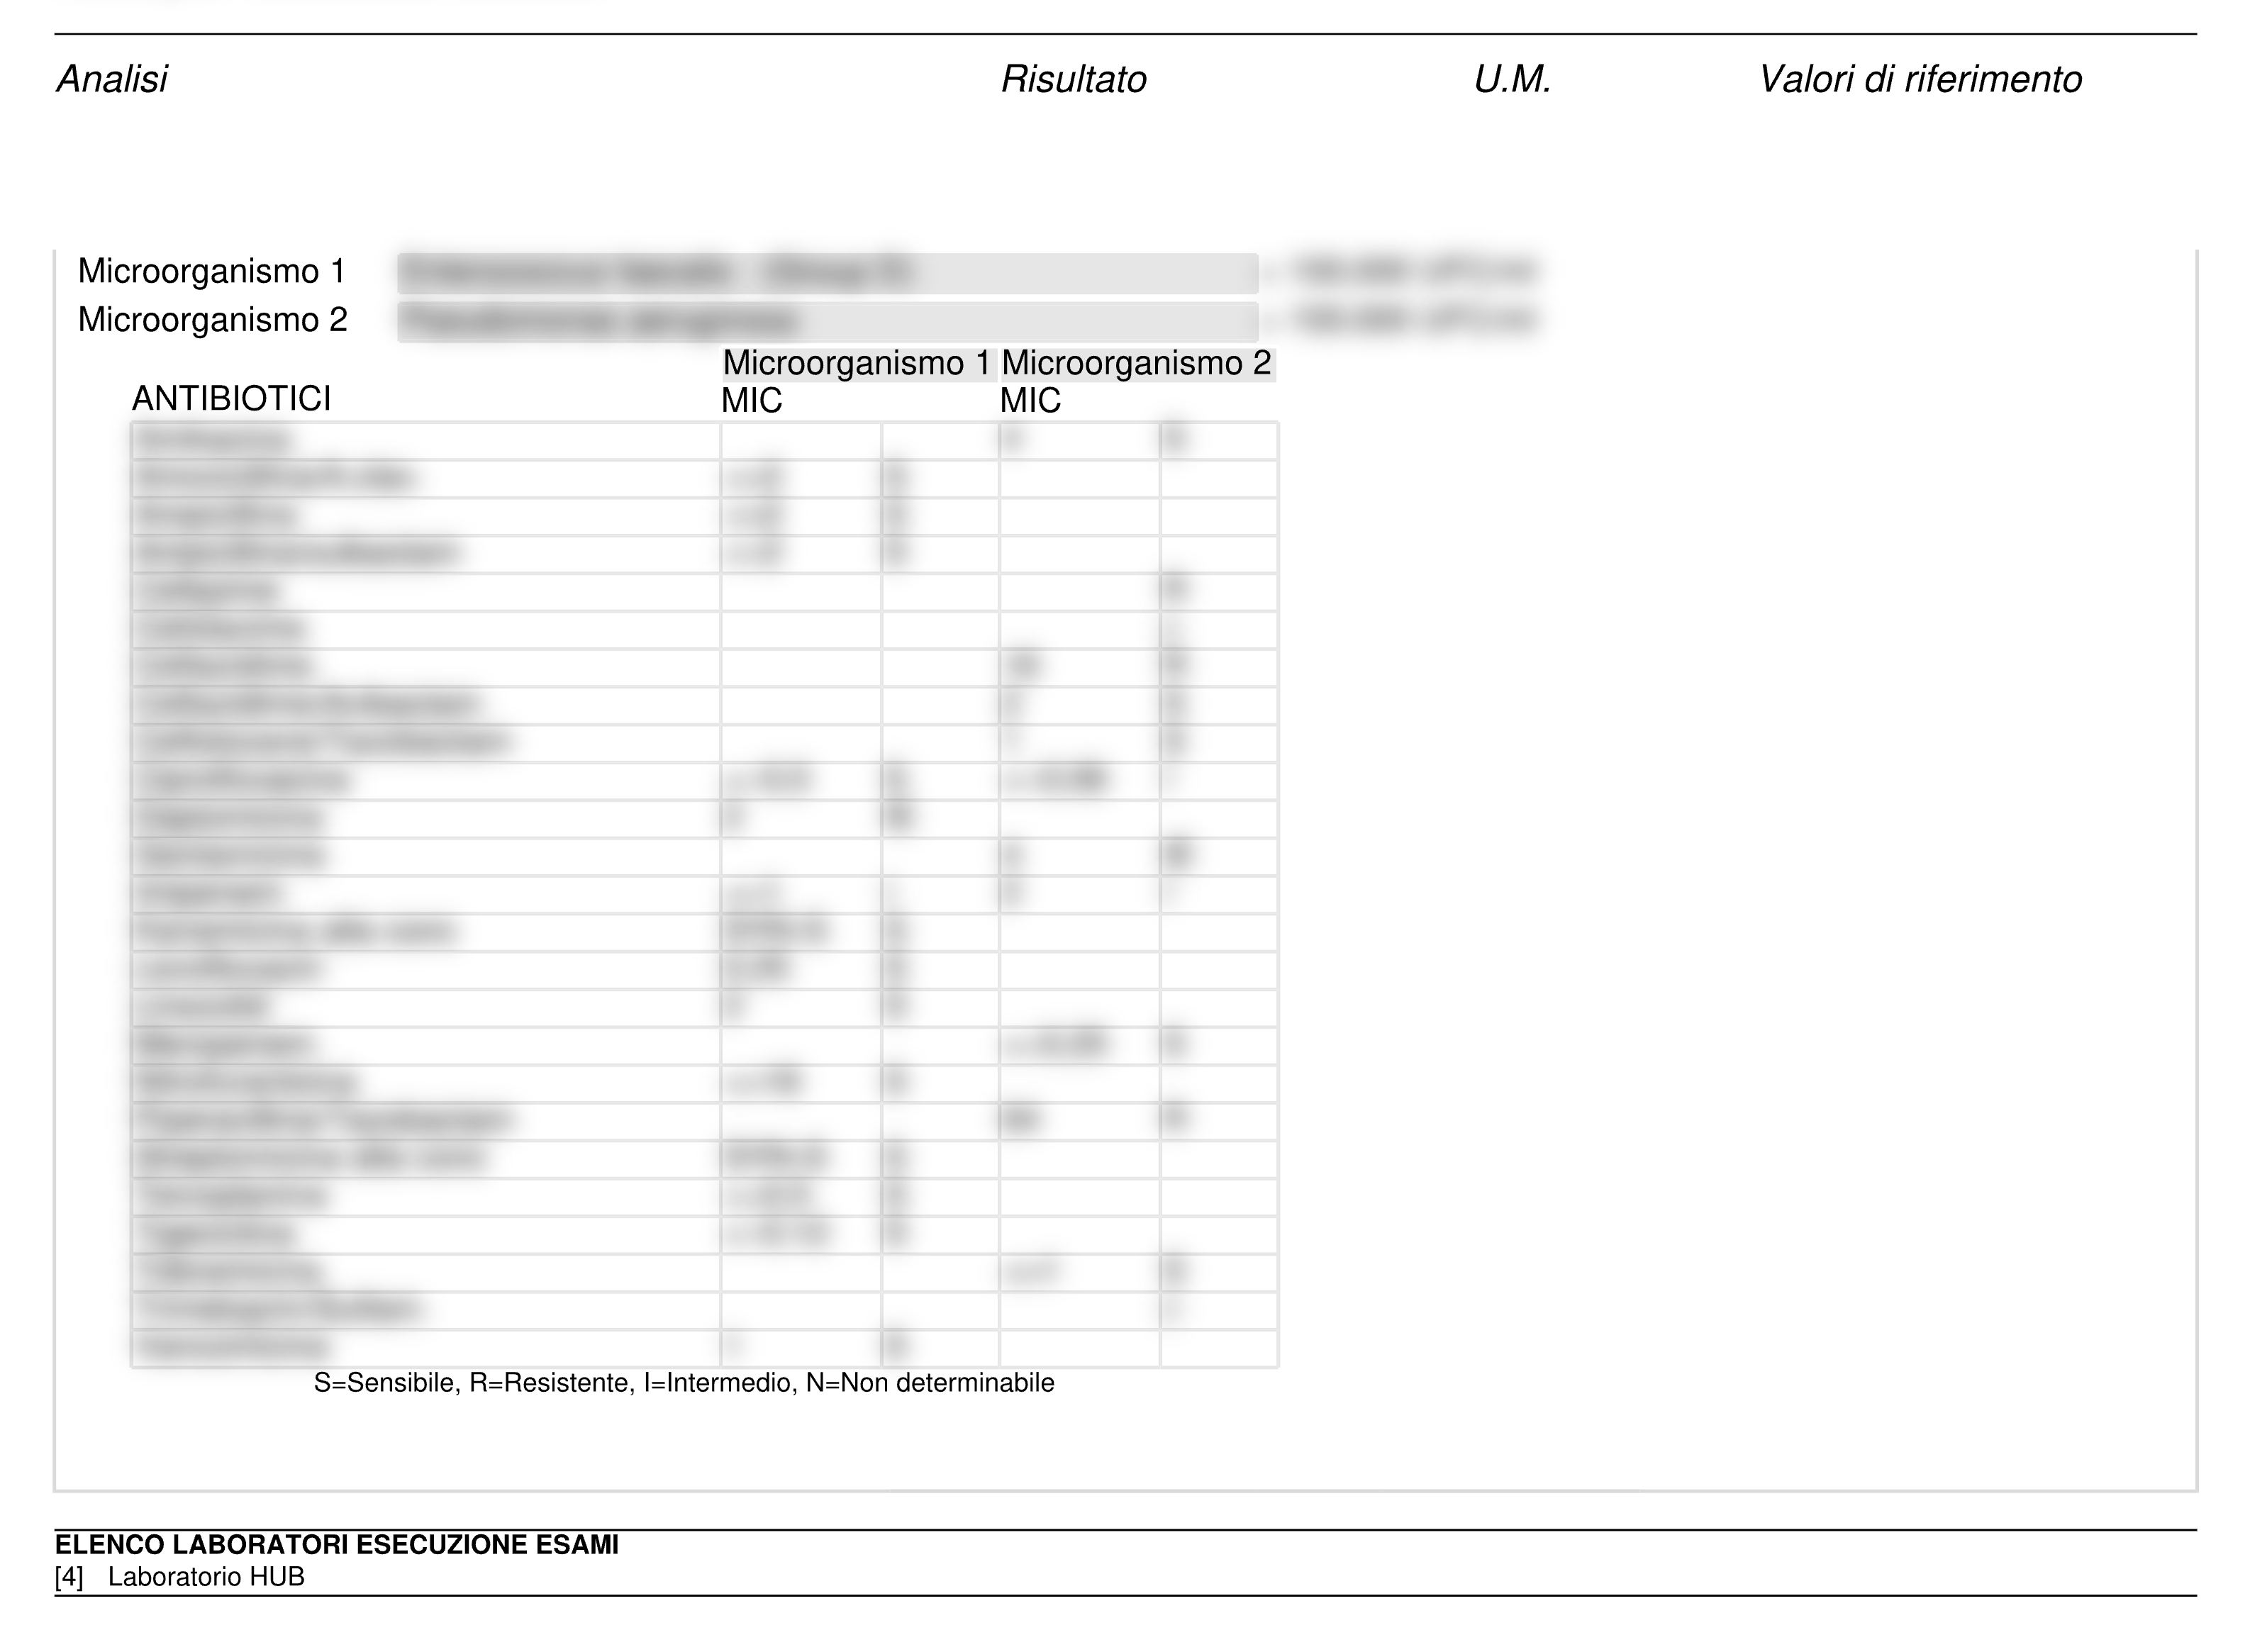
\includegraphics[width=.99\columnwidth]{images/content_multi_p2.png}
	\caption{\textit{}}
	\label{fig:content_multi_2}
\end{figure} 

La tabella in questione non presenta appunto il materiale su cui è basata l'analisi, poichè non è noto l'algoritmo utilizzato per dividere le informazioni si propone una soluzione aggiuntiva, da verificare una volta ottenuti campioni conformi, nella seguente forma algoritmica:
\begin{enumerate}
	\item Per ogni pagina, rimuovere le sezioni:
	\begin{enumerate}
		\item \textit{Intestazione} (fig. \ref{fig:header})
		\item \textit{Anagrafica} (fig. \ref{fig:content})	
		\item \textit{Piè di Pagina} (fig. \ref{fig:content})
	\end{enumerate}	
	\item Unire le pagina in una sola
	\item Procedere dal punto 1) dell'algoritmo proposto nel paragrafo \ref{Algoritmo finale}
\end{enumerate}







